\documentclass[../main.tex]{subfiles}
\begin{document}
In the last 50 years car have transitioned from being composed only by mechanical parts to being completely stacked with electronics. The complexity of vehicles arises every year and the industry continuously raise the bar on the state of the arts. The transitions to electro-mobility, the ADAS systems have done all but slowing down the development. The more a topic is market relevant, the higher the competition between companies, the faster the development in that field is going to be. The automakers are always ready to exploit or create new needs in order to adapt and attract customers. Automotive pulse of innovation and the "German Silicon Valley" is the place a engineer want to be to fell part of this complex, but for sure perfectly oiled, machine.   
\begin{figure}
\centering
\begin{minipage}{.5\textwidth}
  \centering
  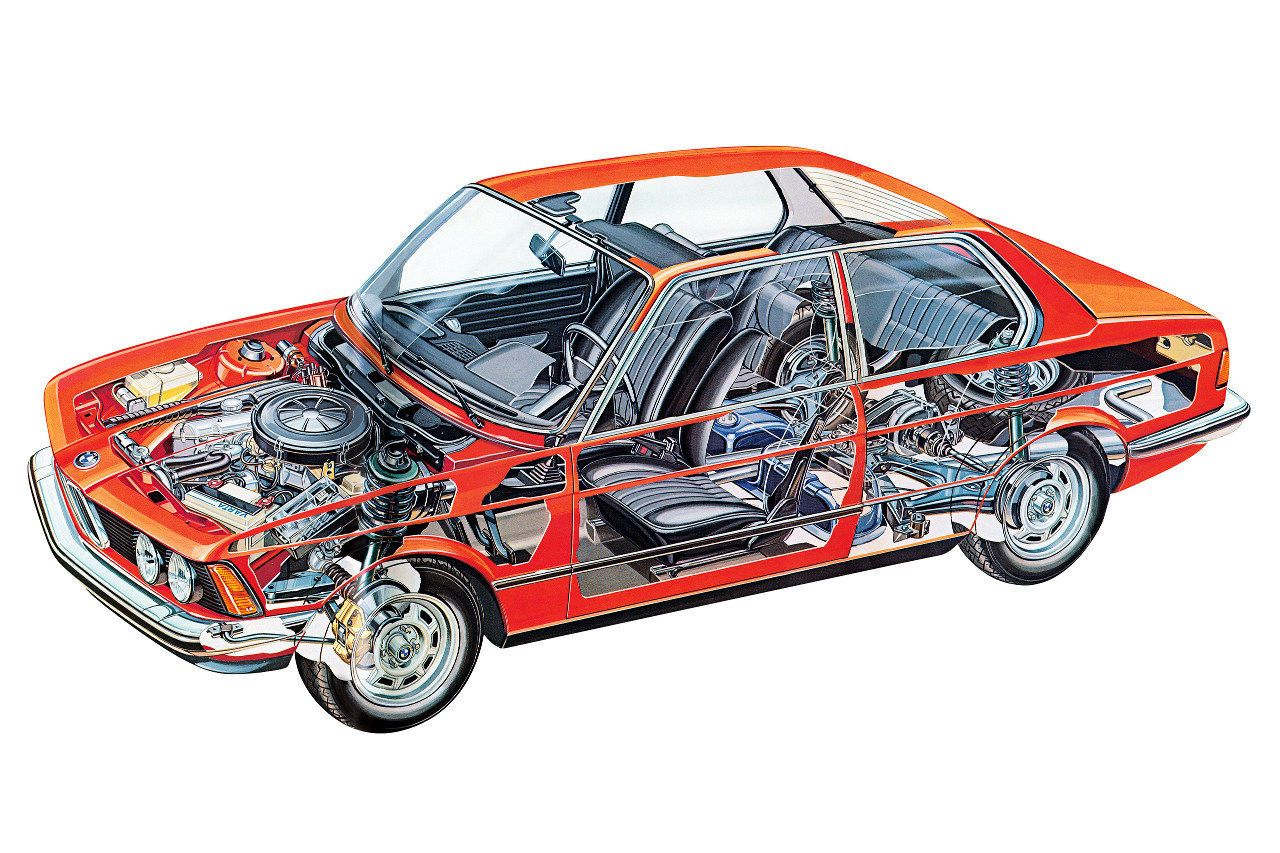
\includegraphics[width=\linewidth]{images_folder/4a56e1d50b56da42a10e29d451cf2b93.jpg}
  \caption{BMW 320 Coupe - 1975}
  \label{fig:test1}
\end{minipage}%
\begin{minipage}{.5\textwidth}
  \centering
  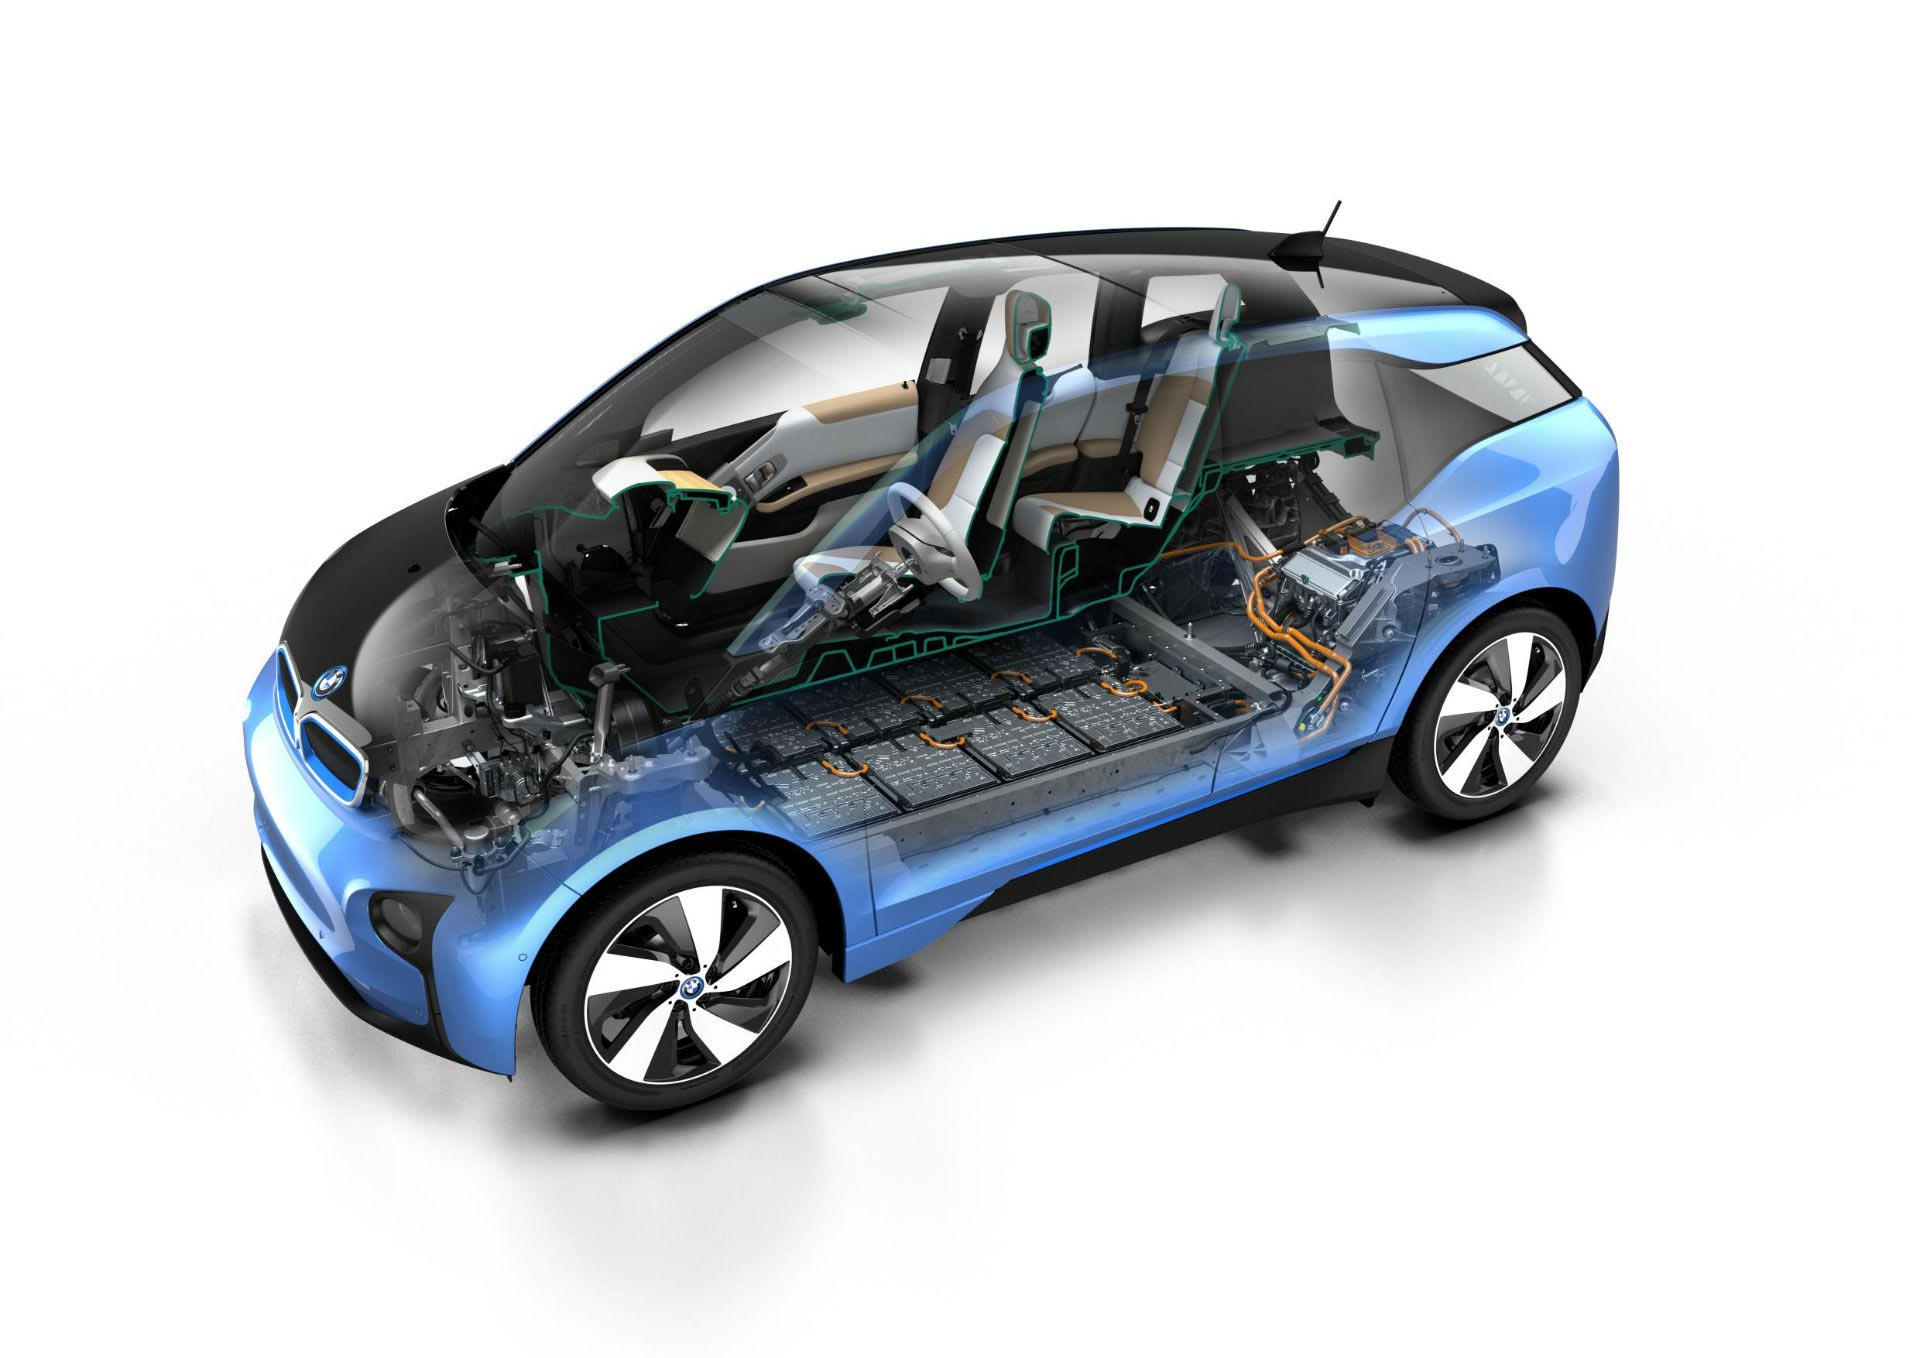
\includegraphics[width=\linewidth]{images_folder/BMW_i3.jpg}
  \caption{BMW I3 - 2015}
  \label{fig:test2}
\end{minipage}
\end{figure}

\section{Block Schema of a car}
The complexity of system car can be easily simplified by block schemes. Block schemes are going to be a recursive topic during the thesis, thanks to the outside view that allow to have on complex topics. 

The input to the car block can be an array of driver commands, such as the steering position, accelerator pressure and all the switches that control the car. The output of the system is the movement of the car, the feedback loop report to the user not only the position in space but also parameters as the drive comfort or the temperature in the vehicle. The car block can therefor be inspect further. Inside the system car we can identify two main blocks. The mechanical one and the electrical one. We can see how feedback loop start to intersect with each other. The electronics drive the mechanics which output is taken back to the electronic to correct the response. The system car can be considered a complex version of an embedded system where electronics drive mechanics following a logic described in lines of code.
Inside the automotive world the trend that has drawn more differences in the way car are constructed is in the electronic components side. if the cost related to the development of mechanical components, safety features and logistic increased constantly through the years, the cost related to the electronic components exponentially increased. Every mechanical component in cars has probably some electronic hardware related to it which is controlled by one of the many ECUs (Electronic control Units) in the vehicle. The increase in hardware requires an increase in the software in order to control it. The yearly increase in lines of code for cars reported in \ref{fig:yearlyincreas} is a statement supporting of the importance of software. 
\begin{figure}[H]
    \centering
    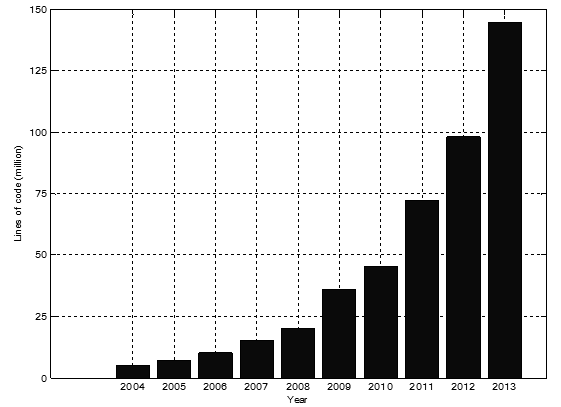
\includegraphics[width=\linewidth]{images_folder/Yearly-increase-in-automotive-software-complexity-shown-by-million-lines-of-code-of-1-ConvertImage.png}
    \caption{Yearly increase in automotive software complexity}
    \label{fig:yearlyincreas}
\end{figure}
The brain of a modern car is represented by the combination of all the different ECUs, providing control for the different parts, from the motor to the door control. 
\section{Software and ECUs}
The development of Software for ECUs is an extremely complex task, a single ECU can control up to a 1000 functions, and the number can be also higher for the control of complex systems, such as the motor. The other big problem is that the function need to be developed in order to work together 
\cleardoublepage
\end{document}